\documentclass[aspectratio=169,11pt]{beamer}
\usetheme{Madrid}
\usecolortheme{default}

% Core packages
\usepackage{amsmath,amssymb}
\usepackage{tikz-cd}
\usepackage{multicol}
\usepackage{graphicx}
\usepackage{xcolor}
\usepackage{booktabs}

% A clean accent color used for "Our Focus" highlights
\definecolor{accentgold}{RGB}{184,134,11}
\definecolor{accentblue}{RGB}{43,74,122}
\definecolor{accentgreen}{RGB}{45,90,61}
\definecolor{accentred}{RGB}{139,38,53}

% Tighten up bullets a bit
\setbeamertemplate{itemize items}[circle]
\setbeamerfont{itemize/enumerate body}{size=\small}
\setbeamerfont{itemize/enumerate subbody}{size=\footnotesize}

\title[Interpreting Medical VLMs with SAEs]{Knowledge-Anchored Sparse Autoencoders \\ for Interpreting Medical Vision-Language Models}
\author{Akib}
\institute{Department of Computer Science and Engineering \\ Islamic University of Technology (IUT)}
\date{\today}

\begin{document}

% =====================================================
\begin{frame}
    \titlepage
\end{frame}

% =====================================================
\begin{frame}{Introduction}
    \textbf{Medical Vision-Language Models (Medical VLMs)}

    \vspace{0.4em}
    \textbf{Definition:} \\
    A Medical VLM is a multimodal neural system that jointly processes a medical image (e.g., chest X-ray) and a natural-language prompt, and produces a textual output such as a finding description, a draft radiology report, or an answer to a clinical question.

    \vspace{0.8em}
    \textbf{Example:} Given a frontal chest X-ray and the prompt \textit{``Describe the findings in this image''}, a model such as LLaVA-Med or CheXagent generates free-form text such as: \textit{``There is increased opacity in the right lower lobe consistent with consolidation. No pleural effusion or pneumothorax.''}

    \vspace{0.8em}
    \textbf{Goal of interpretability for Medical VLMs:} \\
    Not to improve accuracy per se, but to make the model's internal computations inspectable --- so that when the model generates a finding, we can identify \emph{which internal features} caused it, and whether the same features cause hallucinated findings when they should not.
\end{frame}

% =====================================================
\begin{frame}{Problem Statement}
    \textbf{The precise statement of the problem}

    \vspace{0.4em}
    Let $V$ be the vision encoder of a medical VLM. For an input image $x$, $V$ produces a dense activation vector $h \in \mathbb{R}^d$ at a chosen layer, where individual neurons are \emph{polysemantic} --- each mixes several unrelated concepts.

    \vspace{0.4em}
    Let $\mathcal{C} = \{c_1, \dots, c_K\}$ be a set of named clinical concepts obtained from a structured knowledge source (e.g., RadGraph entities extracted from MIMIC-CXR reports).

    \vspace{0.4em}
    A \textbf{Sparse Autoencoder (SAE)} $f$ re-expresses $h$ as an overcomplete, mostly-zero vector $z \in \mathbb{R}^D$ with $D \gg d$, where each non-zero entry of $z$ is intended to correspond to a single interpretable concept.

    \vspace{0.4em}
    \textbf{Problem:} SAEs trained in the standard unsupervised way (Bricken et al. 2023; Pach et al. 2025) produce features whose meanings must be \emph{guessed} post-hoc by inspecting top-activating images --- a procedure known to be unreliable (Stevens et al., 2025).

    \vspace{0.4em}
    \textbf{Task:} Determine whether biasing SAE training with the symbolic concept set $\mathcal{C}$ as an auxiliary signal yields features that are (a) more reliably aligned with named clinical concepts, (b) causally faithful under intervention, and (c) useful for explaining specific hallucination types in medical VLM outputs.
\end{frame}

% =====================================================
\begin{frame}{Motivation}
    \textbf{Where existing work stands --- and what is driving this research}

    \vspace{0.5em}
    \begin{itemize}
        \item \textbf{Medical VLMs are entering clinical pipelines}, but routinely hallucinate: they fabricate findings that are not present, omit findings that are, or misstate severity. In a clinical setting these errors directly threaten patient safety.

        \item \textbf{Current medical interpretability work is dominated by saliency maps.} Saporta et al. (Nature MI 2022) showed that chest-X-ray saliency methods substantially under-perform expert radiologists for pathology localization --- pretty heatmaps are not clinically reliable explanations.

        \item \textbf{Mechanistic interpretability (SAEs, causal interventions) is the current frontier for general-domain VLMs} (Pach et al. NeurIPS 2025; Zaigrajew et al. ICML 2025), but has barely been applied to medical VLMs --- only one close precedent exists (SAE-Rad, 2024).

        \item \textbf{Existing unsupervised SAEs rely on post-hoc guessing of feature meaning.} The ``Brazil/lamp'' finding of Stevens et al. (2025) shows this guessing is frequently wrong. In medicine, where feature meaning has clinical consequences, this failure mode is unacceptable.

        \item \textbf{Our opening:} inject a clinical knowledge graph directly into SAE training so that features carry \emph{names} by construction, not by post-hoc inspection --- and evaluate causally rather than by visual plausibility.
    \end{itemize}
\end{frame}

% =====================================================
\begin{frame}{Objectives}
    \textbf{Primary impact, and secondary contributions}

    \vspace{0.5em}
    \textbf{Impact (the reason this matters):}
    \begin{itemize}
        \item Produce a \emph{clinically inspectable} interpretability tool for medical VLMs, where internal features carry named clinical concepts rather than requiring expert guess-work.
        \item Shift medical VLM explanation from \emph{saliency plausibility} to \emph{mechanistic accountability} --- enabling diagnosis of \textit{why} a hallucination occurred, not just that one occurred.
        \item Provide an open-source toolkit that other medical AI labs can reuse on their own VLMs, raising the methodological floor for clinical interpretability.
    \end{itemize}

    \vspace{0.5em}
    \textbf{Contributions (the technical deliverables):}
    \begin{itemize}
        \item A \textbf{knowledge-anchored SAE training objective} that couples standard reconstruction + sparsity losses with an auxiliary concept-alignment loss driven by RadGraph-derived clinical labels.
        \item A \textbf{three-axis evaluation protocol} for medical interpretability: concept purity, causal faithfulness, and hallucination-diagnostic utility.
        \item An \textbf{empirical comparison} between unsupervised and knowledge-anchored SAEs on an open medical VLM (LLaVA-Med) using MIMIC-CXR and the MedVH hallucination benchmark.
        \item \textbf{Public release} of trained SAEs, code, and the evaluation harness.
    \end{itemize}
\end{frame}

% =====================================================
\begin{frame}{Literature Review --- Taxonomy and Chronology}
    \vspace{-0.4em}
    \begin{center}
        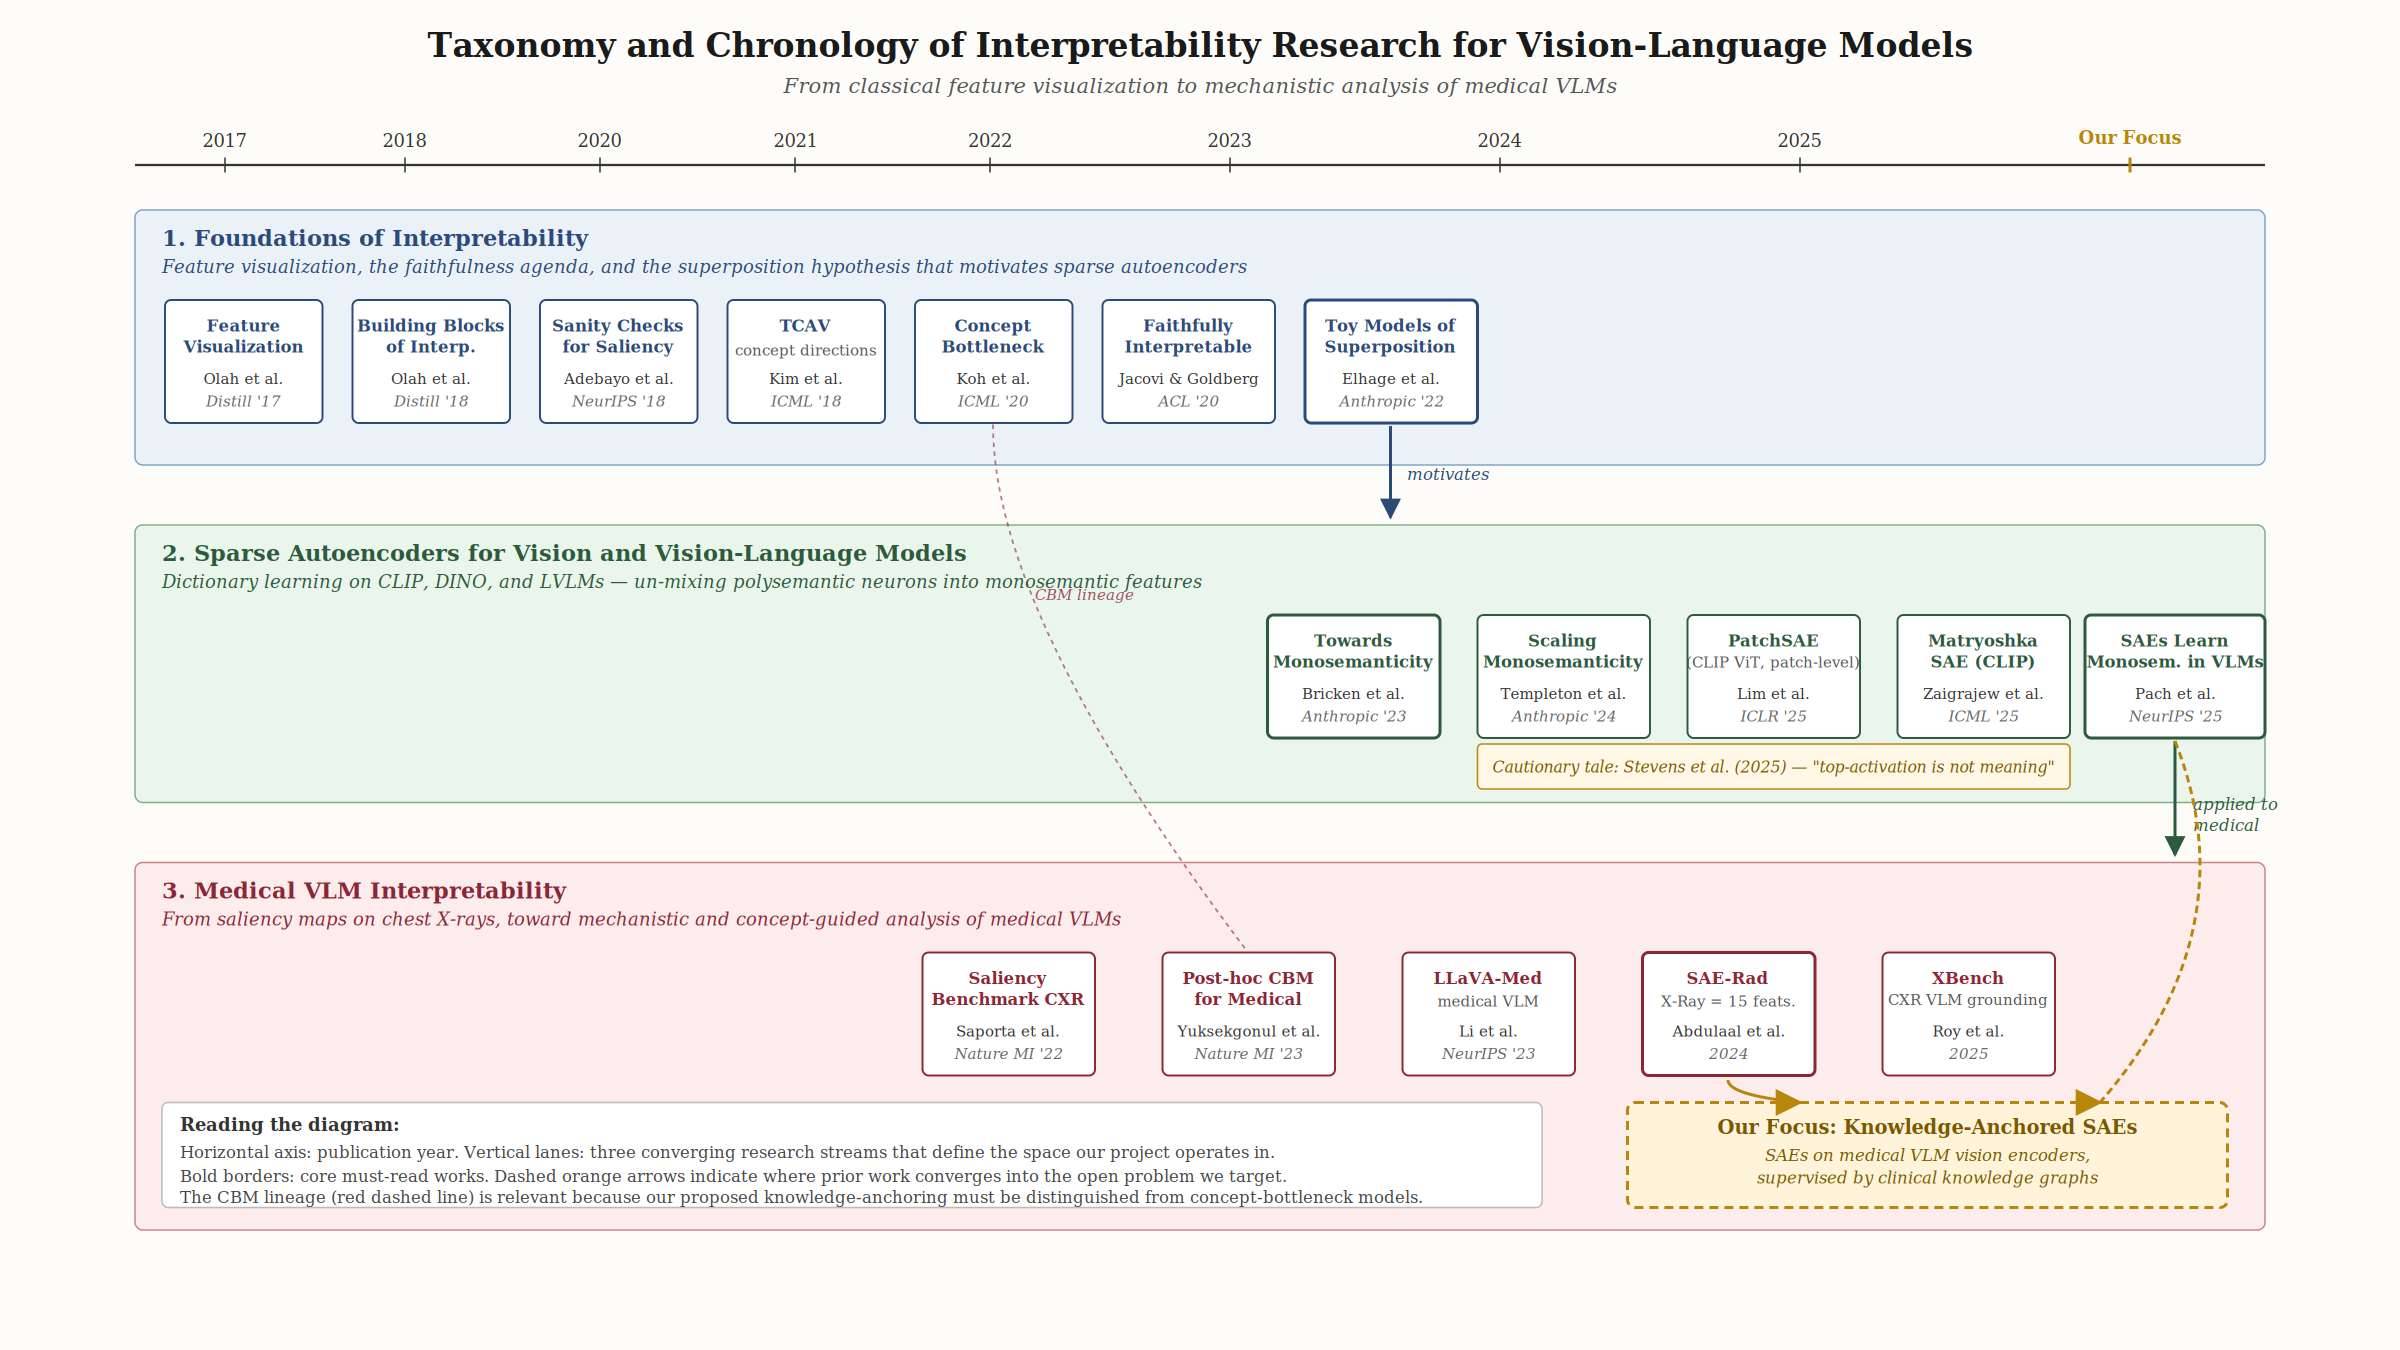
\includegraphics[width=0.98\linewidth]{taxonomy_chronology.png}
    \end{center}

    \vspace{-0.6em}
    \begin{columns}
        \column{0.5\textwidth}
        \footnotesize
        \textbf{The story of the diagram:}
        \begin{itemize}
            \setlength\itemsep{0.1em}
            \item[\textcolor{accentblue}{\textbullet}] Interpretability matured from saliency into the \emph{superposition} hypothesis (Elhage '22).
            \item[\textcolor{accentgreen}{\textbullet}] Sparse autoencoders operationalized that hypothesis for CLIP and general VLMs (Bricken '23 → Pach '25).
        \end{itemize}

        \column{0.5\textwidth}
        \footnotesize
        \textbf{}
        \begin{itemize}
            \setlength\itemsep{0.1em}
            \item[\textcolor{accentred}{\textbullet}] In the medical domain, the leap from saliency to SAEs has barely begun (only SAE-Rad, 2024).
            \item[\textcolor{accentgold}{\textbullet}] Our focus: close this gap with a \emph{knowledge-anchored} variant, explicitly distinguished from Concept Bottleneck Models.
        \end{itemize}
    \end{columns}
\end{frame}

% =====================================================
\begin{frame}{Literature Review --- Foundations of Interpretability}
    \textbf{Five works that set up the intellectual stage}

    \vspace{0.4em}
    \small
    \begin{itemize}
        \item \textbf{Olah et al., \textit{Feature Visualization} (Distill 2017)} --- Systematized activation maximization. Established the language of ``what input most excites this unit?'' that still underlies modern feature discovery.

        \item \textbf{Olah et al., \textit{Building Blocks of Interpretability} (Distill 2018)} --- Proposed that interpretability should be composable: attribution + feature visualization + matrix factorization. Anticipated the modular structure of today's mechanistic toolkit.

        \item \textbf{Adebayo et al., \textit{Sanity Checks for Saliency Maps} (NeurIPS 2018)} --- Delivered the field's most important negative result: many popular saliency methods are nearly unchanged when the model's weights are randomized --- i.e., they are not actually explaining the model. Set the standard that ``looks reasonable'' is no longer acceptable.

        \item \textbf{Koh et al., \textit{Concept Bottleneck Models} (ICML 2020)} --- Argued that interpretability should be \emph{architectural} rather than post-hoc: route predictions through editable human-named concepts. This is the lineage our ``knowledge-anchored SAE'' must clearly differ from.

        \item \textbf{Elhage et al., \textit{Toy Models of Superposition} (Anthropic 2022)} --- Formalized \emph{why} individual neurons are messy: networks pack more features than they have neurons (``superposition''). Directly motivated Sparse Autoencoders as the tool to un-mix them.
    \end{itemize}
\end{frame}

% =====================================================
\begin{frame}{Literature Review --- Sparse Autoencoders for Vision and VLMs}
    \textbf{From language SAEs to multimodal interpretability}

    \vspace{0.4em}
    \small
    \begin{itemize}
        \item \textbf{Bricken et al., \textit{Towards Monosemanticity} (Anthropic 2023)} --- The first clearly successful SAE on a production model. Established the training recipe (overcomplete dictionary + L1 sparsity + MSE reconstruction) that all subsequent work builds on.

        \item \textbf{Templeton et al., \textit{Scaling Monosemanticity} (Anthropic 2024)} --- Scaled SAEs to Claude 3 Sonnet. Demonstrated \emph{feature steering} (suppress or amplify a feature to change behavior) as a real interpretability lever, not only a visualization trick.

        \item \textbf{Lim et al., \textit{PatchSAE} (ICLR 2025)} --- Trained SAEs at the \emph{patch} level of CLIP ViT, enabling spatially-localized concept attribution rather than image-global features --- directly relevant for grounding to anatomical regions.

        \item \textbf{Zaigrajew et al., \textit{Matryoshka SAE for CLIP} (ICML 2025)} --- Hierarchical SAE architecture that captures concepts at multiple levels of abstraction simultaneously, improving both sparsity and reconstruction.

        \item \textbf{Pach et al., \textit{SAEs Learn Monosemantic Features in VLMs} (NeurIPS 2025)} --- The current reference point for vision-language SAEs. Introduces a monosemanticity benchmark grounded in a large-scale user study, and shows that SAE interventions on a CLIP vision encoder can steer downstream LLaVA outputs.

        \item \textcolor{accentgold}{\textbf{Cautionary tale --- Stevens et al. (2025):}} SAE features labeled by top-activating images can be misleading (the ``Brazil'' feature was actually firing on \emph{lamps}). Direct motivation for our causal-evaluation protocol and for anchoring features to a symbolic concept source.
    \end{itemize}
\end{frame}

% =====================================================
\begin{frame}{Literature Review --- Medical VLM Interpretability}
    \textbf{Where the domain actually stands --- and the gap we enter}

    \vspace{0.3em}
    \small
    \begin{itemize}
        \item \textbf{Saporta et al., \textit{Benchmarking Saliency for CXR} (Nature MI 2022)} --- Across seven saliency methods on chest radiographs, performance was substantially below expert radiologists for pathology localization. Cautionary foundation: saliency alone is not clinically trustworthy.

        \item \textbf{Yuksekgonul et al., \textit{Post-hoc Concept Bottleneck for Medical} (Nature MI 2023)} --- Retrofitted CBMs onto trained medical models by mapping representations to clinical concepts such as ``pleural effusion''. The closest precedent for our idea of concept-anchoring --- and the method we must clearly differ from.

        \item \textbf{Li et al., \textit{LLaVA-Med} (NeurIPS 2023)} --- The primary open medical VLM: a CLIP-style vision tower biomedically pretrained on PMC-15M, adapted with instruction-tuning on GPT-4-generated multimodal dialogues. Likely base model for our experiments.

        \item \textbf{Abdulaal et al., \textit{SAE-Rad} (2024)} --- The only prior work applying SAEs to a medical vision model. Showed that 15 sparse features suffice for interpretable X-ray representation, but training is purely unsupervised --- features still require post-hoc guessing.

        \item \textbf{Roy et al., \textit{XBench} (2025)} --- First systematic benchmark for crossmodal interpretability of CXR VLMs. Finding: grounding degrades sharply for small or diffuse lesions. Proves the evaluation gap our work sits inside.
    \end{itemize}

    \vspace{0.3em}
    \textbf{Evaluation-rigor anchors (Phase 5 reading):} Jacovi \& Goldberg (ACL 2020) on faithfulness; Heimersheim \& Nanda (2024) on activation patching as causal evaluation.
\end{frame}

% =====================================================
\begin{frame}{Literature Review --- The Gap We Target}
    \textbf{What prior work does \emph{not} give us}

    \vspace{0.5em}
    \begin{itemize}
        \item General-VLM SAE work (Pach et al., Zaigrajew et al.) is \emph{unsupervised} and \emph{non-medical} --- features carry no clinical names by construction.

        \item Medical CBM work (Yuksekgonul et al.) is \emph{concept-routed at prediction time}, not feature-level. It replaces the model's output layer; it does not un-mix the vision encoder's internal activations.

        \item SAE-Rad applies SAEs to medical images but \emph{inherits the unsupervised guessing problem} --- feature identities are still guessed from top activations, a procedure known to fail (Stevens et al.).

        \item XBench measures \emph{grounding} (spatial faithfulness) but not \emph{mechanistic} accountability (which internal component caused the output).
    \end{itemize}

    \vspace{0.6em}
    \textcolor{accentgold}{\textbf{The opening:}} No existing work simultaneously (a) trains SAEs on a medical VLM's vision encoder, (b) biases training with a clinical knowledge graph so that features are \emph{named by construction}, and (c) evaluates the resulting features causally rather than by visual inspection.

    \vspace{0.3em}
    This is the three-way intersection our project occupies.
\end{frame}

% =====================================================
\begin{frame}{Research Trajectory --- From Literature to Our Contribution}
    \textbf{The convergence argument in one slide}

    \vspace{0.5em}
    \begin{center}
    \begin{tabular}{@{}p{0.3\linewidth}p{0.62\linewidth}@{}}
        \toprule
        \textbf{Stream} & \textbf{Contribution to our approach} \\
        \midrule
        Foundations &
        Supplies the superposition hypothesis (why features must be un-mixed) and the faithfulness bar (why causal evaluation is mandatory). \\
        \addlinespace
        General VLM SAEs &
        Supplies the technical recipe for training SAEs on CLIP-style vision encoders, and a cautionary tale about naive feature interpretation. \\
        \addlinespace
        Medical VLM interp. &
        Supplies the domain constraints (clinical label schema, available open models, MIMIC-CXR ecosystem) and proof that saliency-only methods fail here. \\
        \addlinespace
        CBM lineage &
        Supplies the concept-anchoring idea at prediction-layer granularity --- which we re-deploy at feature-layer granularity through SAE latents. \\
        \bottomrule
    \end{tabular}
    \end{center}

    \vspace{0.6em}
    \textbf{Our position:} the intersection of these four streams, specifically targeted at hallucination diagnosis --- a clinical need that none of the four streams individually addresses.
\end{frame}

% =====================================================
\begin{frame}{What Comes Next in This Deck (Placeholder Sections)}
    \textbf{The following sections are intentionally left for real work}

    \vspace{0.5em}
    These sections will be filled in after the corresponding experimental and methodological work is completed. They are \emph{not} written today because that would mean inventing content that does not yet exist.

    \vspace{0.6em}
    \begin{itemize}
        \item \textbf{Proposed Method} --- SAE architecture, auxiliary-loss formulation, training protocol on LLaVA-Med's vision encoder.
        \item \textbf{Dataset and Preprocessing} --- MIMIC-CXR with RadGraph parses; concept vocabulary from the 14-label CheXpert schema and RadGraph observation/anatomy entities.
        \item \textbf{Experimental Setup} --- Baselines (unsupervised SAE, SAE-Rad re-implementation, linear-probe CBM), hyperparameters, compute budget.
        \item \textbf{Evaluation Protocol} --- Concept purity (held-out RadGraph labels), causal faithfulness (activation patching / feature ablation on generation), hallucination diagnosis (MedVH benchmark).
        \item \textbf{Results} --- Numerical comparisons, ablation studies, qualitative feature examples.
        \item \textbf{Limitations and Future Work}.
    \end{itemize}

    \vspace{0.5em}
    \small \textit{Current status: literature review complete (shown in prior slides); reading-phase 1--3 complete per roadmap; experimental setup in progress.}
\end{frame}

% =====================================================
\begin{frame}{References (Representative, Not Exhaustive)}
    \scriptsize
    \begin{multicols}{2}
    \begin{itemize}
        \item Olah et al., \textit{Feature Visualization}, Distill, 2017.
        \item Olah et al., \textit{The Building Blocks of Interpretability}, Distill, 2018.
        \item Adebayo et al., \textit{Sanity Checks for Saliency Maps}, NeurIPS 2018.
        \item Kim et al., \textit{TCAV: Interpretability Beyond Feature Attribution}, ICML 2018.
        \item Koh et al., \textit{Concept Bottleneck Models}, ICML 2020.
        \item Jacovi \& Goldberg, \textit{Towards Faithfully Interpretable NLP Systems}, ACL 2020.
        \item Elhage et al., \textit{Toy Models of Superposition}, Anthropic, 2022.
        \item Saporta et al., \textit{Benchmarking Saliency Methods for Chest X-Ray Interpretation}, Nature Machine Intelligence, 2022.
        \item Bricken et al., \textit{Towards Monosemanticity: Decomposing Language Models with Dictionary Learning}, Anthropic, 2023.
        \item Li et al., \textit{LLaVA-Med: Training a Large Language-and-Vision Assistant for Biomedicine in One Day}, NeurIPS 2023.
        \item Yuksekgonul et al., \textit{Post-hoc Concept Bottleneck Models}, Nature Machine Intelligence, 2023.
        \item Templeton et al., \textit{Scaling Monosemanticity}, Anthropic, 2024.
        \item Abdulaal et al., \textit{SAE-Rad: An X-Ray Is Worth 15 Features}, 2024.
        \item Heimersheim \& Nanda, \textit{How to Use and Interpret Activation Patching}, 2024.
        \item Lim et al., \textit{PatchSAE: Sparse Autoencoders for Spatial Interpretability}, ICLR 2025.
        \item Stevens et al., \textit{SAEs for Scientifically Rigorous Interpretation of Vision Models}, 2025.
        \item Zaigrajew et al., \textit{Interpreting CLIP with Hierarchical Sparse Autoencoders}, ICML 2025.
        \item Pach et al., \textit{Sparse Autoencoders Learn Monosemantic Features in Vision-Language Models}, NeurIPS 2025.
        \item Roy et al., \textit{XBench: Benchmarking Crossmodal Interpretability in CXR VLMs}, 2025.
        \item Jain et al., \textit{RadGraph: Extracting Clinical Entities and Relations from Radiology Reports}, NeurIPS 2021.
        \item Johnson et al., \textit{MIMIC-CXR}, Scientific Data, 2019.
        \item Irvin et al., \textit{CheXpert: A Large Chest Radiograph Dataset}, AAAI 2019.
    \end{itemize}
    \end{multicols}
\end{frame}

% =====================================================
\begin{frame}
    \centering
    \vspace{1.5cm}
    {\LARGE \textbf{Thank you}}

    \vspace{0.8cm}
    {\normalsize Questions and guidance welcome.}
\end{frame}

\end{document}
